\documentclass[
a4paper,					% DINA4 Papier
12pt,						% Schriftgröße 12
oneside,
openany,
parskip=half,				% Abstand nach Absatz (statt Einrückung)
headsepline=true,			% Linie nach Kopfzeile
footsepline=false,			% Linie vor Fußzeile
plainfootsepline=true,		% Linie vor Fußzeile auf \chapter{}-Seiten
listof=totoc,				% Abblidungs- und Tabellenverzeichnis im Imhalsverteichnis darstellen
toc=bibliography,			% Literaturverzeichnis im Inhlatsverzeichnis darstellen
abstract=on,				% Abstract mit Titel
]{scrreprt}					% KOMA-Script-Äquivalent zur Standardklasse report

%%%%%%%%%% Allgemein %%%%%%%%%%%%%%%%%%%%%%%%%%%%%%%%%%%%%%%%%%%%%%%%%%%%%%%%%%%%%%%%%%%%%%%%%%%%%%%

% Einstellungen laden
%%%%%%%%%Allgemeine persönliche Daten (zu ändern)%%%%%%%%%%%%%%%%%%%%%%%%%%%%%%%%%%%%%%%%%%%%
\newcommand{\titel}{Entwurf und prototypische Implementierung eines Sprachassistenzsystemes für ARBURGs Maschinensteuerung GESTICA}
\newcommand{\artDerArbeit}{Praxisarbeit}
\newcommand{\arbeit}{T3\_2000}
\newcommand{\betreuer}{B. Eng., Benedikt Link}
%\newcommand{\betreuerzwei}{ -}
\newcommand{\zeitraum}{KW 23 - KW 40}
\newcommand{\abgabedatum}{04. Oktober 2022}

\newcommand{\matrikelnr}{3758638}
\newcommand{\studiengang}{Informatik}
\newcommand{\kurs}{TINF2020}
\newcommand{\firma}{ARBURG GmbH \& Co KG }
\newcommand{\firmenadresse}{Arthur-Hehl-Straße, 72290 Loßburg}
\newcommand{\abgabeort}{Horb am Neckar}
\newcommand{\dhbw}{Dualen Hochschule Baden-Württemberg Stuttgart Campus Horb}
\newcommand{\autor}{Jonas Weis}

%Bildverzeichnis
\newcommand{\imgpath}{01_img/}

%Code-Verzeichnis
\newcommand{\codepath}{02_code}

%UML-Verzeichnis
\newcommand{\umlpath}{06_uml/}

% Nummerierung in der Bildbeschreibung
\newcommand{\fortlaufendenummerierung}{true}


%%%%%%%%%% Code %%%%%%%%%%%%%%%%%%%%%%%%%%%%%%%%%%%%%%%%%%%%%%%%%%%%%%%%%%%%%%%%%%%%%%%%%%%%%%%%%%%%

% Standard-Monospace-Schriftart
\newcommand{\monofont}{Consolas}


% Breitere Abstände zwischen Wörtern erlauben, um zu breite Zeilen zu vermeiden
% Ähnlich wie sloppypar-Umgebung, wobei diese einen Wert von 3em setzt
\setlength{\emergencystretch}{1em}

% Sprache
\usepackage[english,ngerman]{babel}
\selectlanguage{ngerman}

% Anführungszeichenstil
\usepackage[style=german,german=quotes]{csquotes}

% Lorem Ipsum
\usepackage{lipsum}

% erweiterte Schriftgrößenänderungen
\usepackage{relsize}

% Farben
\usepackage[table, x11names]{xcolor}
\usepackage{transparent}

% Grafiken/Bilder
\usepackage{graphicx}
\graphicspath{{\imgpath}{\umlpath}}
\usepackage{subfig}


% Standalone-Latex-Dateien einbinden
\usepackage{standalone}

%Bild fixieren \FloatBarrier
\usepackage{placeins}

% Programmierte Verktorgrafiken
\usepackage{tikz}
\usetikzlibrary{decorations.pathreplacing}
\usetikzlibrary{backgrounds}
\usetikzlibrary{calc}
\usetikzlibrary{arrows.meta}
\usetikzlibrary{fit}
\usetikzlibrary{shapes}
\usetikzlibrary{positioning}
\usetikzlibrary{arrows}
\usetikzlibrary{decorations.text}
\usetikzlibrary{decorations.pathmorphing}
\usetikzlibrary{automata}

% zusätzliche Aufzählungsarten
\usepackage{paralist}

% zusätzliche Tabellenfunktionen
\usepackage{tabularx}
\usepackage{booktabs}
\usepackage[flushleft]{threeparttable}
\usepackage{ltablex}
\usepackage{multirow}
\usepackage{multicol}
\usepackage{longtable}
\usepackage{makecell}
\usepackage{ltablex}
\keepXColumns
\usepackage{array}
\newcolumntype{I}{>{\labelitemi~~}l<{}}
\newcolumntype{P}[1]{>{\centering\arraybackslash}p{#1}} % Zentral in Zelle mit "P{xcm}"
\newcolumntype{L}[1]{>{\raggedright\arraybackslash}p{#1}} % Links in Zelle mit "L{xcm}"
\newcolumntype{R}[1]{>{\raggedleft\arraybackslash}p{#1}} % Rechts in Zelle mit "R{xcm}"
\newcommand{\talign}[2]{\multicolumn{1}{#1}{#2}}

% zusätzliche Aufzählungen
\usepackage{enumitem}

% mathematische Symbole der American Mathematical Society
\usepackage{amsfonts}
\usepackage{amsmath}

% Berechnungen von Längenangaben
\usepackage{calc}

% Rotation
\usepackage{rotating}

% Querformat für Seiten
\usepackage{pdflscape}

% URLs
\usepackage[hyphens]{url}
\usepackage[anythingbreaks]{breakurl}

% Hypelinks
\usepackage[pdfencoding=auto]{hyperref}
\hypersetup{
	pdftitle={\titel},			% PDF-Titel
	pdfauthor={\autor},			% PDF-Autor
	pdfcreator={LuaLaTeX},
	breaklinks,
	hidelinks,					% Links nicht umrahmen
	bookmarksnumbered=true,		% Überschriftnummerierung im PDF-Inhalt anzeigen
	pageanchor=true				% \autoref und \cite Zahlen auch als Link darstellen
}
\usepackage{bookmark}
\usepackage{nameref}

% Glossar
\usepackage[
toc,				% Verzeichnisse ins Inhaltsverzeichnis aufnehmen
acronym,			% Abkürzungsverzeichnis
nonumberlist,		% keine Seitenzahlen in Verzeichnissen
nogroupskip,		% kein Abstand zwischen Einträgen mit dem gleichen Anfangsbuchstaben
style=long,			% Verzeichnis als longtable darstellen
]{glossaries}
\newglossarystyle{mystyle}{
	\setglossarystyle{long}
	\renewenvironment{theglossary}
	{\begin{longtable}{L{4cm}p{\glsdescwidth+1cm}}
		\renewcommand{\arraystretch}{1.5}}
		{\end{longtable}}
}
\hyphenation{Programmierung} % Ausnahme: Verhindert die Worttrennung von Programmierung (sah im Glossar blöd aus)

\renewcommand{\glsnamefont}[1]{\textbf{#1}}
\newcommand{\glsr}[2][]{
	\glsdisp[#1]{#2}{\glsentryshort{#2} (\glsentrylong{#2})}
}
\setacronymstyle{short-long}	% kurz (lang)
%include pdf to document
\usepackage{pdfpages}

% BibTex
\usepackage[
backend=biber,		% Bibliograhpieprogramm
bibencoding=utf-8,	% Kodierung
sortlocale=de_DE,	% Sortiersprache
bibstyle=ieee,		% Stil des Literaturverzeichnisses
citestyle=numeric,	% Stil der Referenzen (ieee: [1], [2] | numeric: [1, 2])
dashed=false		% true: bei mehreren Quellen mit dem selben Author wird ab dem 2. Mal ein Strich (-----) anstelle des Namens verwendet (nur bei bibstyle=ieee|authoryear nötig)
]{biblatex}
\DefineBibliographyStrings{ngerman}{
	bibliography={Literaturverzeichnis},	% Literaturverzeichnis statt Literatur als Überschrift
	url={[Online]\adddot\addspace URL}								% "URL: http://..." statt "Adresse: http://..." in Quellenangabe
}
\DeclareNameAlias{author}{last-first}						% Nachname vor Vorname
\let\lastnameformat=\textnormal								% Nachname nicht komplett in Großbuchstaben
\DeclareFieldFormat{labelnumberwidth}{\mkbibbrackets{#1}}	% Eckige Klammer in Literaturverzeichnis
\DeclareFieldFormat{shorthandwidth}{\mkbibbrackets{#1}}		% Eckige Klammer bei Zitaten
\urlstyle{same}												% gleiche Schrift für URL
\addbibresource{literatur.bib}								% Literaturdatenbank einbinden


\usepackage{xpatch}
\xpatchbibdriver{online}
{\printtext[parens]{\usebibmacro{date}}}
{\iffieldundef{year}
	{}
	{\printtext[parens]{\usebibmacro{date}}}}
{}
{\typeout{There was an error patching biblatex-ieee (specifically, ieee.bbx's @online driver)}}

\usepackage{xparse}


\newcommand\ddfrac[2]{\frac{\displaystyle #1}{\displaystyle #2}}

%%%%%%%%%% Eigene Environments %%%%%%%%%%%%%%%%%%%%%%%%%%%%%%%%%%%%%%%%%%%%%%%%%%%%%%%%%%%%%%%%%%%%%%%%%%

% Grafiken/Bilder
\usepackage{newfloat}
\DeclareFloatingEnvironment[
fileext=lop,
listname={Diagrammverzeichnis},
name=Diagramm,
placement=tp,
within=none
]{uml}

% Andere
\usepackage{amsthm}
\theoremstyle{definition}
\newtheorem{definition}{Definition}
\theoremstyle{remark}
\newtheorem*{remark}{Anmerkung}

%%%%%%%%%%%%%%%%%%%%%%%%%%%%%%%%%%%%%%%%%%%%%%%%%%%%%%%%%%%%%%%%%%%%%%%%%%%%%%%%%%%%%%%%%%%%%%%%%%%%

\newenvironment{nscenter}
{\parskip=0pt\par\nopagebreak\centering}
{\par\noindent\ignorespacesafterend}

%%%%%%%%%% Formatierungen %%%%%%%%%%%%%%%%%%%%%%%%%%%%%%%%%%%%%%%%%%%%%%%%%%%%%%%%%%%%%%%%%%%%%%%%%%

% Zeilenabstand
%\usepackage[
%singlespacing
%spacing
%doublespacing
%]{setspace}
%\linespread{1.25}
\usepackage{setspace}
\makeatletter
\newcommand{\MSonehalfspacing}{%
	\setstretch{1.25}%  default
	\ifcase \@ptsize \relax % 10pt
	\setstretch {1.25}%
	\or % 11pt
	\setstretch {1.25}%
	\or % 12pt
	\setstretch {1.433}%
	\fi
}
\newcommand{\MSdoublespacing}{%
	\setstretch {1.92}%  default
	\ifcase \@ptsize \relax % 10pt
	\setstretch {1.936}%
	\or % 11pt
	\setstretch {1.866}%
	\or % 12pt
	\setstretch {1.902}%
	\fi
}
\makeatother
\MSonehalfspacing

% Seitenränder und Höhe von Kopf- und Fußzeile
\usepackage[a4paper, left=3cm, right=2.5cm, top=2.5cm, bottom=2.5cm]{geometry}

% Standardschriftart: Helvetica
\usepackage[T1]{fontenc}
\usepackage[scaled]{helvet}
\renewcommand{\familydefault}{\sfdefault}
\usepackage{lmodern}

% Monospace Schriftart definieren
\usepackage{fontspec}
\setmonofont{\monofont}


% Rahmen um Text o.a.
\usepackage{tcolorbox}
\newtcolorbox{myframe}[1][]{
	arc=0pt,
	outer arc=0pt,
	colback=white,
	boxrule=0.8pt,
	#1
}
\usepackage{efbox}

% Nummer der caption ohne Kapitelzahl
\usepackage{chngcntr}

%%%%%%%%%%%%%%%%%%%%%%%%%%%%%%%%%%%%%%%%%%%%%%%%%%%%%%%%%%%%%%%%%%%%%%%%%%%%%%%%%%%%%%%%%%%%%%%%%%%%
% Lückenfüller

\newcommand{\shortlorem}{Lorem ipsum dolor sit amet, consetetur sadipscing elitr, sed diam nonumy eirmod tempor invidunt ut labore et dolore magna aliquyam erat, sed diam voluptua.}
\newcommand{\longlorem}{Lorem ipsum dolor sit amet, consetetur sadipscing elitr, sed diam nonumy eirmod tempor invidunt ut labore et dolore magna aliquyam erat, sed diam voluptua. At vero eos et accusam et justo duo dolores et ea rebum. Stet clita kasd gubergren, no sea takimata sanctus est Lorem ipsum dolor sit amet. Lorem ipsum dolor sit amet, consetetur sadipscing elitr, sed diam nonumy eirmod tempor invidunt ut labore et dolore magna aliquyam erat, sed diam voluptua. At vero eos et accusam et justo duo dolores et ea rebum. Stet clita kasd gubergren, no sea takimata sanctus est Lorem ipsum dolor sit amet.}

%%%%%%%%%% Kopf- und Fußzeile %%%%%%%%%%%%%%%%%%%%%%%%%%%%%%%%%%%%%%%%%%%%%%%%%%%%%%%%%%%%%%%%%%%%%%

\usepackage{scrlayer-scrpage}
\pagestyle{scrheadings}
\clearscrheadfoot
\addtokomafont{pageheadfoot}{\setstretch{1}}
% Abstand zwischen Kopfzeile und \chapter{title}
\renewcommand*{\chapterheadstartvskip}{\vspace*{0.0\baselineskip}}
% kursive Seitenzahl
\renewcommand{\pagemark}{\textit{\thepage}}
% Fußzeile mittig
\cfoot*{\pagemark}
%     ^ Stern: Fußzeile wird auch auf seiten mit \pagestyle{plain} wie z.B. \chapter{title} angezeigt

%%%%%%%%%% Code %%%%%%%%%%%%%%%%%%%%%%%%%%%%%%%%%%%%%%%%%%%%%%%%%%%%%%%%%%%%%%%%%%%%%%%%%%%%%%%%%%%%

\usepackage{caption}
\DeclareCaptionFont{black}{\color{black}}
\DeclareCaptionFormat{listing}{#1#2#3}
\captionsetup[lstlisting]{format=listing, labelfont=black, textfont=black, singlelinecheck=false, margin=0pt, font={bf, footnotesize},} % Change Caption from Code

% Package für Codedarstellung mit Syntax-Highlighting
% Benutzung: 
% \begin{lstlisting}
% 	<Code/>
% \end{lstlisting}
\usepackage{listings}

% Definition eigener Klassen von Schlüsselwörter für das Syntax-Highlighting
\makeatletter
% Klassen
\lst@InstallKeywords k{classes}{classstyle}\slshape{classstyle}{}ld
\makeatother

\newcommand{\keywordstyle}{\color[HTML]{0000ff}}
\newcommand{\commentstyle}{\color[HTML]{228b22}}
\newcommand{\stringstyle}{\color[HTML]{800000}}

% allgemeine Styles

\lstset{language=[Sharp]C,
	numbers=left,
	numberstyle=\tiny\color{white},
	numbersep=5pt,
	tabsize=2,
	extendedchars=true,
	breaklines=true,
	frame=lines,
	showspaces=false,
	showtabs=false,
	xleftmargin=1pt,
	framexleftmargin=1pt,
	framexrightmargin=1pt,
	framexbottommargin=1pt,
	framextopmargin=1pt,
	morecomment=[l]{//}, %use comment-line-style!
	morecomment=[s]{/*}{*/}, %for multiline comments
	showstringspaces=false,
	morekeywords={abstract, as, base, bool, break, byte, case, catch, char, checked, class, const, continue, decimal, default, delegate, do, double, else, enum, event, explicit, extern, false, finally, fixed, float, for, foreach, goto, if, implicit, in, int, interface, internal, is, lock, long, namespace, new, null, object, operator, out, override, params, private, protected, public, readonly, ref, return, sbyte, sealed, short, sizeof, stackalloc, static, string, struct, switch, this, throw, true, try, typeof, uint, ulong, unchecked, unsafe, ushort, using, using, static, virtual, void, volatile, while, add, alias, ascending, async, await, by, descending, dynamic, equals, from, get, global, group, into, join, let, nameof, on, orderby, partial, partial, remove, select, set, value, var, when, where, where, yield, IEnumerable, get, set, List, List<string>, IEnumerable<string>
	},
	moreclasses={ % Klassen angaben, damit dieses mit classescolor hervorgehoben werden
		RecognizedPhrase, ICommandToken, SemanticResultKey, Choices, GrammarBuilder, ILanguage, PanelUris, Grammar, Uri
	},
	stringstyle=\color{gray},
	basicstyle=\fontsize{8}{10}\selectfont\ttfamily\color{black},
	classstyle=\color{Cyan4},
	backgroundcolor=\color{white},
	commentstyle=\color{green},
	keywordstyle=\color{blue},
}

\begin{comment}
	Alternativer Dark-Mode:
	
	\DeclareCaptionFont{white}{\color{white}}
	\DeclareCaptionFormat{listing}{\colorbox{RoyalBlue3}{\parbox{\textwidth}{\hspace{5pt}#1#2#3}}}
	\captionsetup[lstlisting]{format=listing,labelfont=white,textfont=white, singlelinecheck=false, margin=0pt, font={bf,footnotesize}} % Change Caption from Code
	
	
	\lstset{language=[Sharp]C,
		frame=top,frame=bottom,
		numbers=left,
		numberstyle=\tiny\color{white},
		numbersep=5pt,
		tabsize=2,
		extendedchars=true,
		breaklines=true,
		frame=b,
		stringstyle=\color{blue}\ttfamily,
		showspaces=false,
		showtabs=false,
		xleftmargin=1pt,
		framexleftmargin=1pt,
		framexrightmargin=1pt,
		framexbottommargin=1pt,
		commentstyle=\color{green},
		morecomment=[l]{//}, %use comment-line-style!
		morecomment=[s]{/*}{*/}, %for multiline comments
		showstringspaces=false,
		keywordstyle=\color{cyan},
		morekeywords={abstract, as, base, bool, break, byte, case, catch, char, checked, class, const, continue, decimal, default, delegate, do, double, else, enum, event, explicit, extern, false, finally, fixed, float, for, foreach, goto, if, implicit, in, int, interface, internal, is, lock, long, namespace, new, null, object, operator, out, override, params, private, protected, public, readonly, ref, return, sbyte, sealed, short, sizeof, stackalloc, static, string, struct, switch, this, throw, true, try, typeof, uint, ulong, unchecked, unsafe, ushort, using, using, static, virtual, void, volatile, while, add, alias, ascending, async, await, by, descending, dynamic, equals, from, get, global, group, into, join, let, nameof, on, orderby, partial, partial, remove, select, set, value, var, when, where, where, yield, IEnumerable, get, set, List, List<string>, IEnumerable<string>
		},
		moreclasses={													% Klassen angaben, damit dieses mit classescolor hervorgehoben werden
			RecognizedPhrase, ICommandToken, SemanticResultKey, Choices, GrammarBuilder, ILanguage, PanelUris, Grammar, Uri
		},
		stringstyle=\color{Chocolate3},
		basicstyle=\fontsize{8}{10}\selectfont\ttfamily\color{white},
		classstyle=\color{Aquamarine3},
		backgroundcolor=\color{darkgray},
	}
\end{comment}

\lstdefinestyle{xml}{
	language={XML},
	morestring=[b]",
	morecomment=[s]{<?}{?>},
	morecomment=[s]{<!--}{-->},
	stringstyle=\color[HTML]{99401d},
	tagstyle=\color[HTML]{002385},
	keywordstyle=\color[HTML]{808080},
	commentstyle=\commentstyle,
	morekeywords={xmlns,version,type,standalone,name,kid,activityCondition,textResource},	% list your attributes here
	%moreidentifiers={PanelGroup,SectionGroup,TableGroup,ColumnGroup,ParameterItem}
}

\lstdefinelanguage{go}{
	morekeywords=[1]{package,import,func,type,struct,return,defer,panic,recover,select,var,const,iota,},%
	morekeywords=[2]{string,uint,uint8,uint16,uint32,uint64,int,int8,int16,int32,int64,bool,float32,float64,complex64,complex128,byte,rune,uintptr,error,interface},%
	morekeywords=[3]{map,slice,make,new,nil,len,cap,copy,close,true,false,delete,append,real,imag,complex,chan,},%
	morekeywords=[4]{for,break,continue,range,go,goto,switch,case,fallthrough,if,else,default,},%
	morekeywords=[5]{Println,Printf,Error,Print,},%
	sensitive=true,%
	morecomment=[l]{//},%
	morecomment=[s]{/*}{*/},%
	morestring=[b]',%
	morestring=[b]",%
	morestring=[s]{`}{`},%
	keywordstyle=\keywordstyle,
	commentstyle=\commentstyle,
	stringstyle=\stringstyle,
}

\newcommand\YAMLcolonstyle{\color{gray}\mdseries}
\newcommand\YAMLvaluestyle{\stringstyle\mdseries}
\lstdefinelanguage{yaml}{
	sensitive=false,
	keywords={true,false,null,y,n},
	comment=[l]{\#},
	morestring=[b]',
	morestring=[b]",
	moredelim=**[il][\YAMLcolonstyle{:}\YAMLvaluestyle]{:},
	keywordstyle=\keywordstyle,
	commentstyle=\commentstyle,
	stringstyle=\YAMLvaluestyle,
}

\lstdefinelanguage{ebnf}{
	keywords={grammar,parser,lexer},
	morecomment=[l]{//},
	morecomment=[s]{/*}{*/},
	morestring=[b]',
	literate=*{
		{+}{{{\color[HTML]{dd0000}+}}}1
		{*}{{{\color[HTML]{dd0000}*}}}1
		{?}{{{\color[HTML]{dd0000}?}}}1
		{|}{{{\color[HTML]{44bbcc}|}}}1
	},
	keywordstyle=\keywordstyle,
	commentstyle=\commentstyle,
	stringstyle=\stringstyle,
}

\lstdefinestyle{bash}{
	language={bash},
	keywordstyle=\keywordstyle,
	commentstyle=\commentstyle,
	stringstyle=\stringstyle,
}

\lstdefinelanguage{pseudo}{
	mathescape=true,
	morekeywords={input, output, variables, return, begin, end, do, while, if, else, func, new, push, pop, append},
	keywordstyle=\keywordstyle,
}
\lstdefinelanguage{regex}{
	literate=*{
		{a-z}{{{\keywordstyle{}a-z}}}3
		{A-Z}{{{\keywordstyle{}A-Z}}}3
		{0-9}{{{\keywordstyle{}0-9}}}3
		{*}{{{\stringstyle{}*}}}1
		{?}{{{\stringstyle{}?}}}1
		{+}{{{\stringstyle{}+}}}1
		{|}{{{\commentstyle{}|}}}1
		{\{}{{{\commentstyle{}\{}}}1
		{\}}{{{\commentstyle{}\}}}}1
	},
}



\definecolor{eclipseStrings}{RGB}{42,0.0,255}
\definecolor{eclipseKeywords}{RGB}{127,0,85}
\colorlet{numb}{magenta!60!black}

\lstdefinelanguage{json}{
	commentstyle=\color{eclipseStrings}, % style of comment
	stringstyle=\color{eclipseKeywords}, % style of strings
	string=[s]{"}{"},
	comment=[l]{:\ "},
	morecomment=[l]{:"},
	literate=
	*{0}{{{\color{numb}0}}}{1}
	{1}{{{\color{numb}1}}}{1}
	{2}{{{\color{numb}2}}}{1}
	{3}{{{\color{numb}3}}}{1}
	{4}{{{\color{numb}4}}}{1}
	{5}{{{\color{numb}5}}}{1}
	{6}{{{\color{numb}6}}}{1}
	{7}{{{\color{numb}7}}}{1}
	{8}{{{\color{numb}8}}}{1}
	{9}{{{\color{numb}9}}}{1}
}
% zusätzliche Symbolzeichen
\usepackage{textcomp}

% Code--Benennung
\renewcommand{\lstlistingname}{Quellcode}
% Listsings-Verzeichnis umbenennen
\renewcommand{\lstlistlistingname}{Quellcodeverzeichnis}
% Inline Code
\DeclareRobustCommand{\code}[1]{{%
		\begingroup%
		\setlength{\fboxsep}{2pt}%
		\colorbox[HTML]{f3f4f4}{\texttt{\color[HTML]{24292e}\vphantom{Ay}{\smaller\detokenize{#1}}}}%
		\endgroup%
}}


%%%%%%%%%% Util %%%%%%%%%%%%%%%%%%%%%%%%%%%%%%%%%%%%%%%%%%%%%%%%%%%%%%%%%%%%%%%%%%%%%%%%%%%%%%%%%%%%

\usepackage[prependcaption,textsize=small]{todonotes}
\presetkeys{todonotes}{linecolor=yellow,backgroundcolor=yellow!25,bordercolor=yellow}{}

%%%%%%%%%%%%%%%%%%%%%%%%%%%%%%%%%%%%%%%%%%%%%%%%%%%%%%%%%%%%%%%%%%%%%%%%%%%%%%%%%%%%%%%%%%%%%%%%%%%%

% Abkürzungen
\newacronym{arburg}{ARBURG}{ARBURG GmbH \& Co KG}

\newacronym{gestica}{GESTICA}{GESTICA Maschinensteuerung}

\newacronym{selogica}{SELOGICA}{SELOGICA Maschinensteuerung}

\newacronym{cca}{CCA}{Composite Components Architecture}

\newacronym{coco}{CoCo}{Composite Components}

\newacronym{mvvm}{MVVM}{Model-View-ViewModel}

\newacronym{xaml}{XAML}{Extensible Application Markup Language}

\newacronym{wpf}{WPF}{Windows Presentation Foundation}

\newacronym{ui}{UI}{User Interface}

\newacronym{api}{API}{Application Programming Interface}

\newacronym{clr}{CLR}{Common Language Runtime}

\newacronym{sdk}{SDK}{Software Development Kit}

\newacronym{oop}{OOP}{Objektorientierte Programmierung}

\newacronym{linq}{LINQ}{Language Integrated Query}

\newacronym{di}{DI}{Dependency Injection}


%%%%%%%%%%%
% Glossar % %%%%%%%%%%%%%%%%%%%%%
%%%%%%%%%%%
\newglossaryentry{freeformer}{name={Freeformer},description={Maschine zur additiven Fertigung von Kunststoffbauteilen}}

\newglossaryentry{allrounder}{name={ALLROUNDER},description={Spritzgießmaschine zur Kunststoffverarbeitung}}

\newglossaryentry{framework}{name={Framework},description={Programmiergerüst der Softwareentwicklung}}

\newglossaryentry{opensource}{name={Open Source},description={Software, deren Quelltext eingesehen, genutzt und verändert werden darf}}

\newglossaryentry{dotnet_framework}{name={.NET},description={Das vereinheitlichte Framework zur Entwicklung auf Microsoft-Betriebssystemen}}

\newglossaryentry{wrapper}{name={Wrapper},description={Ein Adapter, welcher eine Software umgibt um Kompatibilitäts-, Sicherheits- oder architiktonische Probleme zu lösen}}

\newglossaryentry{class_diagram}{name={Klassendiagramm},description={Statisches Diagramm zur Darstellung von Klassen, Schnittstellen und Beziehungen}}

\newglossaryentry{sequence_diagram}{name={Sequenzdiagramm},description={Interaktions-Diagramm zur zeitlich korrekten Darstellung von Abläufen zwischen Objekten}}

\newglossaryentry{interface}{name={Interface},description={Schnittstelle zur Definition von Methoden und Attributen, welche in einer Klasse vorhanden sein müssen}}

\newglossaryentry{getter}{name={Getter},description={Zugriffsfunktion zur Abfrage des Wertes eines Attributes}}

% Datei erzeugen
\makeglossaries

\ihead{\headmark}
\automark{chapter}
\usepackage{amssymb}


\begin{document}
	% Abbildungen u.Ä.: forlaufende Nummerierung statt Nummerierung pro Kapitel
\newboolean{fortnum}
\setboolean{fortnum}{\fortlaufendenummerierung}
\ifthenelse{\boolean{fortnum}}{
	\counterwithout{figure}{chapter}
	\counterwithout{table}{chapter}
	\counterwithout{lstlisting}{chapter}
	% needed because otherwise table numering starts with the number of the chapter the fist table is in
	% (reason unknown)
	\setcounter{table}{0}
}{}

	
	\begin{titlepage}
		%%start titlepage here
\newgeometry{
left=25mm,
right=25mm,
top=25mm,
bottom=25mm,
headsep=0mm,
footskip=0mm
}
\setstretch {1.25}
\begin{minipage}[ht]{35mm}
	
\includegraphics[width=35mm]{logo_dhbw}
\end{minipage}
\hfill
\begin{minipage}[ht]{30mm}
	
\includegraphics[width=35mm]{logo_arburg}
\end{minipage}
\begin{center}
	\vspace{4.5\baselineskip}
	\LARGE{\textbf{\titel}}\\
	\vspace{1.5\baselineskip}
	\large{\textbf{\artDerArbeit}}\\
	\large\textbf{\arbeit}
	\vspace{1.0\baselineskip}

	des Studiengangs \studiengang an der\\ 
	\dhbw
	\vspace{1.0\baselineskip}
	
	von\\
	\autor \\
	\vspace{1.0\baselineskip}
	\abgabedatum
	\vspace{2.5\baselineskip}
\end{center}

\begin{flushleft}
	\centering
	\begin{tabular}{llll}
		\textbf{Bearbeitungszeitraum} &  & \quad\quad\quad\quad\quad\zeitraum & \\
		\textbf{Matrikelnummer} & & \quad\quad\quad\quad\quad\matrikelnr &\\
		\textbf{Kurs} & & \quad\quad\quad\quad\quad\kurs &\\
		\textbf{Ausbildungsfirma} & & \quad\quad\quad\quad\quad\firma &\\
		& & \quad\quad\quad\quad\quad\firmenadresse&\\
		\textbf{Betreuer} & & \quad\quad\quad\quad\quad\betreuer &\\
		%\textbf{2. Betreuer:} & & \quad\quad\quad\quad\quad\betreuerzwei&\\
	\end{tabular}
\end{flushleft}
	\end{titlepage}
	\pagenumbering{Roman}
	%%%%%%%Sperrvermerk%%%%%%%%%%%%%%%%%%%%%%
\chapter*{Sperrvermerk}
% \addcontentsline{toc}{chapter}{Sperrvermerk}
\thispagestyle{plain}

\begin{tcolorbox}[
	width=\linewidth,
	colframe=red,
	colback=white,
	sharp corners,
	boxrule=1mm,
	halign=center
	]{
	\large Der Inhalt dieser Arbeit darf weder als Ganzes noch in Auszügen Personen außerhalb des Prüfungsprozesses und des Evaluationsverfahrens zugänglich gemacht werden, sofern keine anderslautende Genehmigung der Firma \firma vorliegt.}

%\vspace{20mm}
\end{tcolorbox}

	\chapter*{Eidesstattliche Erklärung}
% \addcontentsline{toc}{chapter}{Eidenstattliche Erklärung}  
\thispagestyle{plain}

gemäß § 5 (4) der „Studien- und Prüfungsordnung DHBW Technik“
vom 14. Juli 2021.
Ich versichere hiermit, dass ich meine Projektarbeit mit dem Thema
\begin{center}
	\textbf{\titel}
\end{center}
selbstständig verfasst und keine anderen als die angegebenen Quellen und Hilfsmittel benutzt habe.\\
\mbox{}
\vfill
\begin{tabularx}{\linewidth}{lXr}
	Loßburg, den \today 		& & 
\includegraphics[width=\linewidth/4]{Unterschrift} \\
%	\cline{1-2}
%	\cline{4-5}
	\rule{50mm}{0.4pt} 			& & \rule{50mm}{0.1pt}\\
	{\footnotesize Ort,Datum}	& & {\footnotesize Unterschrift}\\\end{tabularx}	
	%%%%%%%%%Abstract (Kurzzusammenfassung)%%%%%%%%%%%%%%%%
% Aufbau eines Abstracts (allgemein):
% - eigenständig verständliche
% - 150-250 Wörter (max. 1 Seite)
% - beinhaltet: Fragestellung, Vorgehensweise, Hauptergebnis
% - W-Fragen beantworten: Worum geht es? Wie wurde vorgegangen? Was ist das Ergebnis/was bedeutet es?

% Inhalt (konkret):


\begin{abstract}
	\thispagestyle{plain}
	\addcontentsline{toc}{chapter}{Zusammenfassung}
	
\end{abstract}
\glsresetall

\begin{otherlanguage}{english}
	\begin{abstract}
		\thispagestyle{plain}
		\addcontentsline{toc}{chapter}{Abstract}
		
	\end{abstract}
\end{otherlanguage}
\glsresetall

	\newpage
	\pdfbookmark[chapter]{\contentsname}{toc} % Inhaltsverzeichnis als Lesezeichen in der PDF
	\tableofcontents
	{
		\renewcommand{\addvspace}[1]{\vspace{0mm}}
		\printglossary[style={mystyle}, type=\acronymtype, title={Abkürzungsverzeichnis}] % Abkürzungen
		\printglossary[style={mystyle}] % Erklärungen
		\listoffigures % Bilder
		\listoftables % Tabellen
		\lstlistoflistings % Quellcode
		\clearpage
	}
	
	% Seitennummer speichern und mit normalem von 0 beginnen
	\newcounter{TmpPage}
	\setcounter{TmpPage}{\value{page}}
	\pagenumbering{arabic}
	\setcounter{table}{0}
	
	% WICHTIG: Tatsächlicher Content in passender Reihenfolge einbinden
	\chapter{Einleitung}
\label{chap:einleitung}
Dieses Kapitel gibt eine Übersicht über das Unternehmen \gls{arburg}. Nachfolgend wird die Aufgabenstellung aufgezeigt, deren Motivation erklärt sowie die Vorgehensweise geplant. 

\section{Unternehmensportrait}
\label{sec:unternehmen}
Das Familienunternehmen \gls{arburg} wurde 1923 von Arthur Hehl gegründet. Mittlerweile ist \gls{arburg} einer der weltweit führenden Hersteller von Spritzgießmaschinen zur Kunststoffverarbeitung. Das Stammwerk mit einer Fläche von 210.000 Quadratmetern befindet sich in Loßburg und ist Arbeitsplatz von rund 2.900 Mitarbeitern. Es handelt sich um den einzigen Produktionsstandort. Der Eigenfertigungsanteil der Produktion liegt bei circa 60\%. An knapp 100 Standorten weltweit sind insgesamt rund 600 weitere Mitarbeiter für Service, Vertrieb und Beratung angestellt. 2021 betrug der konsolidierte Umsatz 735 Millionen Euro. Im Portfolio von ARBURG befinden sich elektrische, hybride und hydraulische Spritzgießmaschinen (siehe \autoref{fig:maschinen} a), die \gls{allrounder} genannt werden. Außerdem zugehörige Peripherie und Robot-Systeme. Im Bereich der additiven Fertigung ergänzt seit 2013 der \gls{freeformer} (siehe \autoref{fig:maschinen} b) das Angebot der Firma.

\begin{figure}[!htb] 
	\centering
	\subfloat[\centering Spritzgießmaschine \gls{allrounder}]{{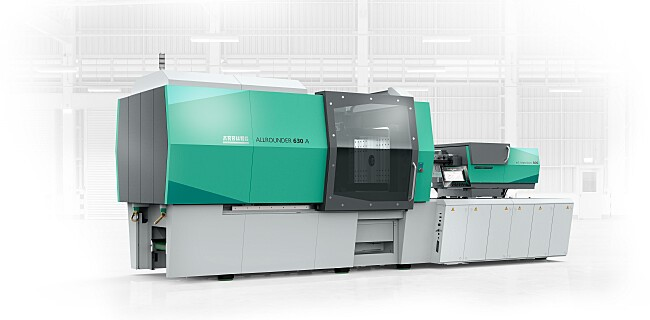
\includegraphics[width=7.8cm]{spritzgiessmaschine.jpg}}}%
	\qquad
	\subfloat[\centering \gls{freeformer}]{{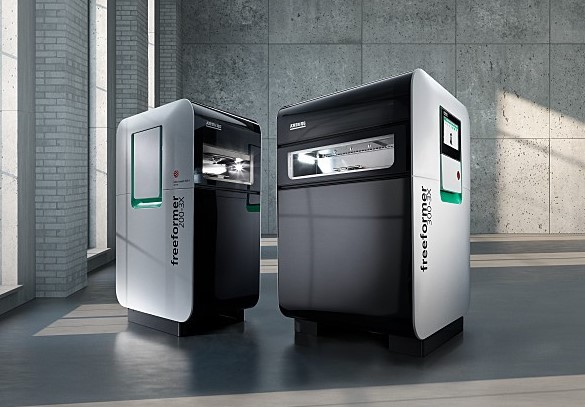
\includegraphics[width=5.5cm]{freeformer.jpg}}}%
	\caption{Produkte der Firma \gls{arburg} \cite{ARBURGGmbH+CoKG_Mediendatenbank}}%
	\label{fig:maschinen}%
\end{figure}
\FloatBarrier

Zur Bedienung der Maschinen ist die \gls{selogica} und seit 2016 auch die \gls{gestica} (siehe \autoref{fig:gestica_steuerung}) in Verwendung.

\begin{figure}[!htb] 
	\centering
		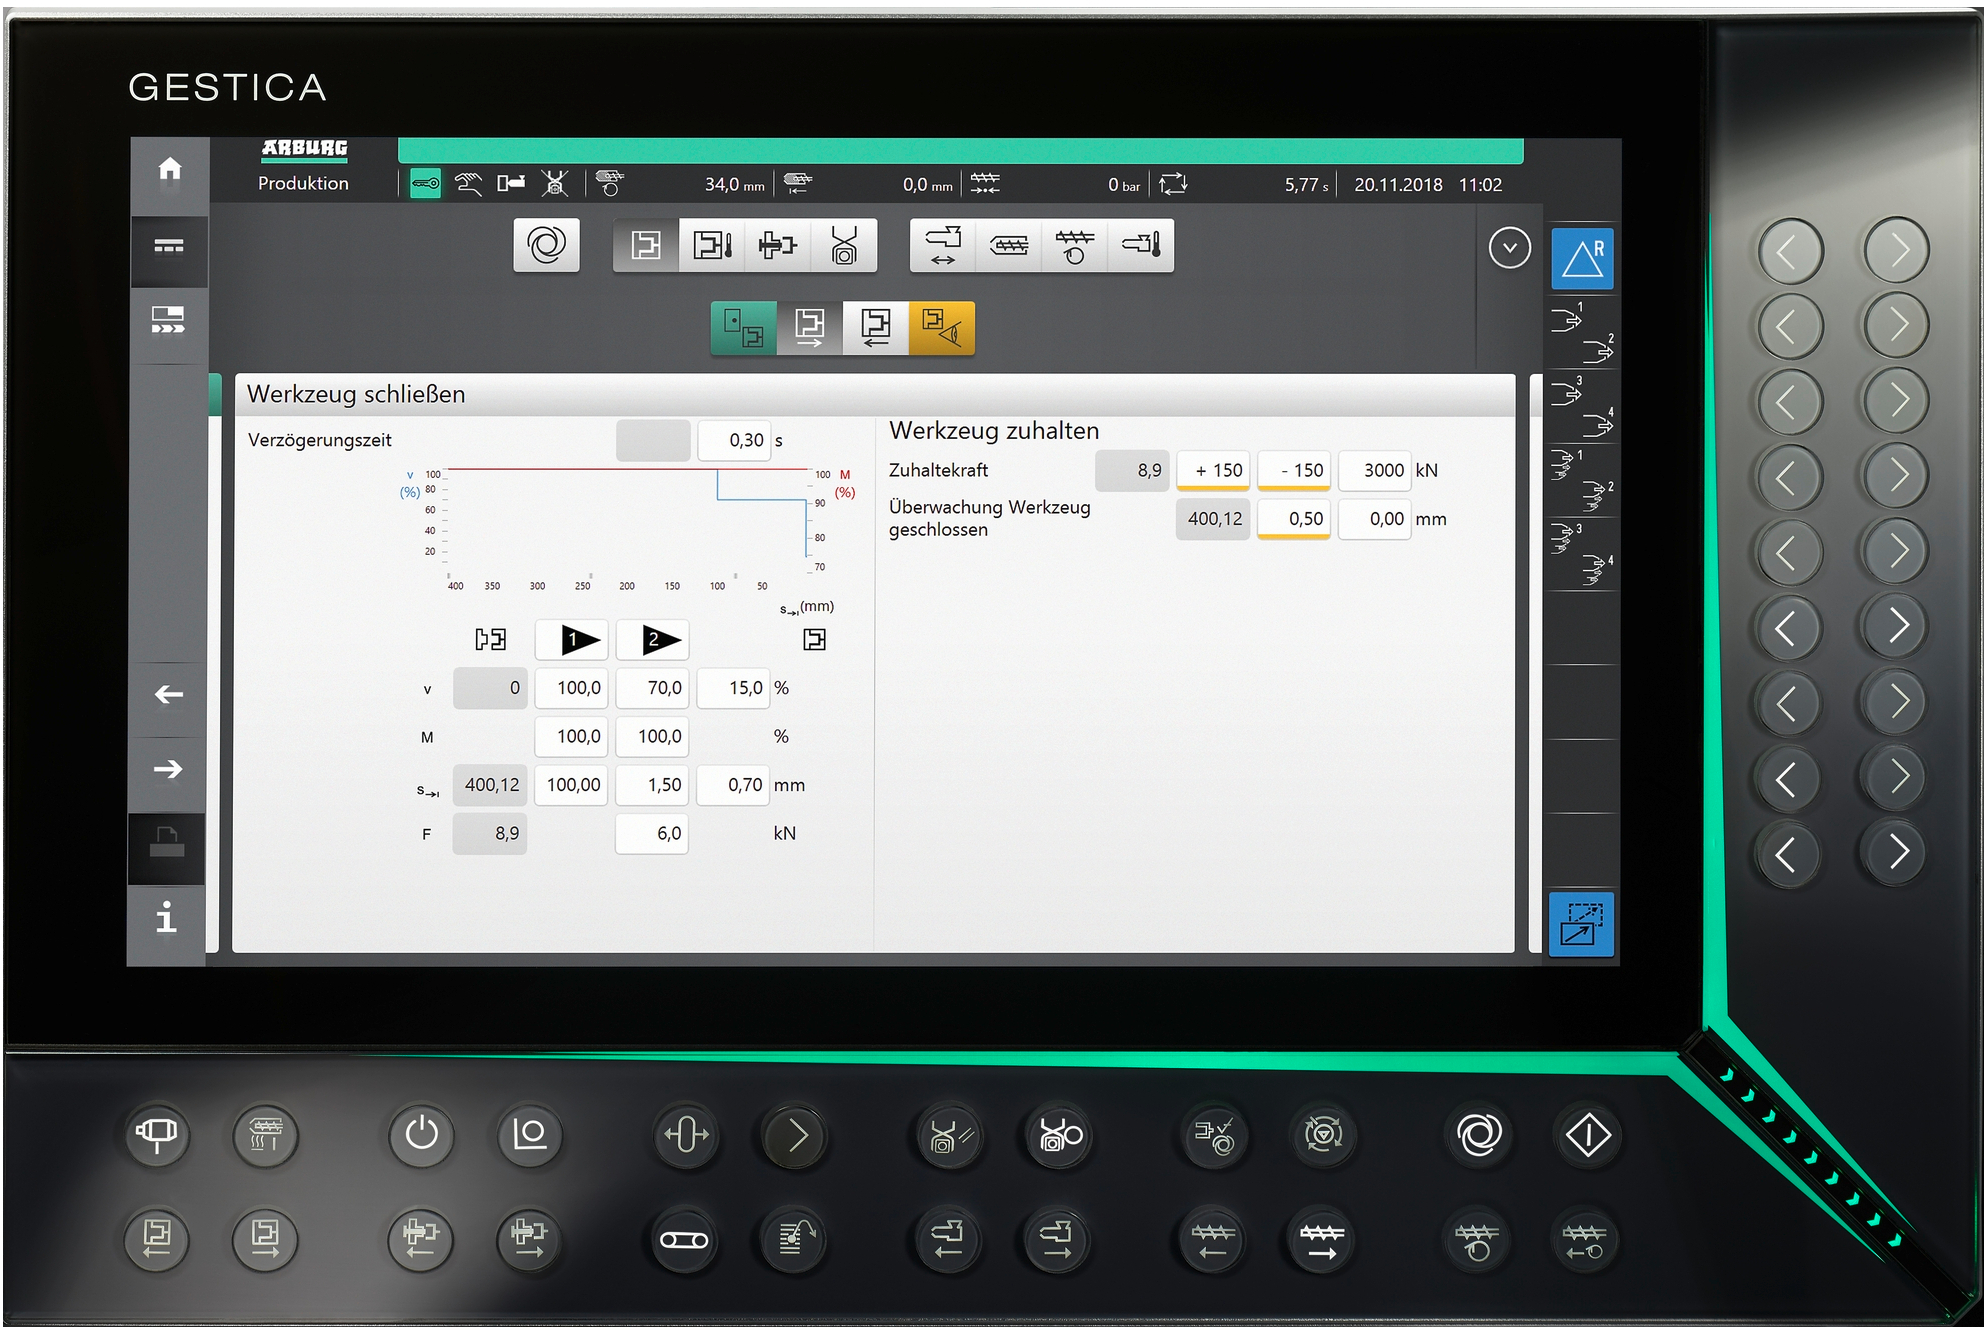
\includegraphics[width=8cm]{gestica.jpg}
	\caption{\gls{gestica} \cite{ARBURGGmbH+CoKG_Mediendatenbank}}
	\label{fig:gestica_steuerung}
\end{figure}
\FloatBarrier

\section{Motivation}
\label{motivation}
Seit Jahren nimmt die Spracherkennung- und Steuerung eine größere werdende Rolle ein. Bereits 2019 nutzen in Deutschland 51 Prozent der 18-24 Jährigen und etwa ein Drittel der 25-64 Jährigen einen Sprachassistenten per Smartphone \cite{Sprachassisten.2019}. Der Absatz von intelligenten Lautsprechern hat sich seit Anfang 2017 mehr als verzehnfacht \cite{SmarteLautsprecher.2021}. Auch im Unternehmen \gls{arburg} besteht der Wunsch, die Steuerung der Maschinen durch eine Sprachsteuerung zu verbessern. Aktuell ist dies nicht möglich. Dieser Wunsch ergibt sich aus dem Vorsatz, der Konkurrenz stets einen Schritt voraus zu sein und den aktuellen Stand der Technik voranzubringen. Grundgedanke ist die einfachere und schnellere Bedienung der Maschine für den Nutzer. Je nach Konzeption entfällt die Notwendigkeit für freie und saubere Hände, was die Wartung erleichtert. Die Implementierung eines solchen Features bietet dem Kunden einen Mehrwert und kann somit mehr Umsatz generieren. 

\section{Aufgabenstellung und Vorgehensweise}
\label{sec:aufgabevorgehen}
Aufgabe ist es, eine Sprachsteuerung für die \gls{arburg}-Maschinen zu konzeptionieren. Zunächst gibt eine Literaturrecherche Aufschluss darüber, wie verschiedene Spracherkennungen in der Theorie funktionieren und welche Chancen und Probleme dort auftreten können. Folgend werden unterschiedliche Anforderungen an ein Sprach-\gls{framework} definiert. Anhand dieser folgt eine Analyse verschiedener Software auf ihre Eignung. Schließlich findet die Auswahl der geeignetsten für die Nutzung im Hause \gls{arburg} statt. Außerdem werden Anforderungen für das Konzept der Sprachsteuerung definiert. Dies geschieht mithilfe des Befragens von Service-Technikern und Mitarbeitern des Schulungscenters. Diese haben zum einen direkten Kontakt mit dem Kunden und dessen Wünschen. Zum anderen kennen sie sich mit der Maschine aus und können daher die Sinnhaftigkeit verschiedener Ideen abschätzen. Dabei ist es nicht vorgesehen, jede Aktion auch durch einen Sprachbefehl ausführen zu können. Hier muss abgegrenzt werden, was sinnvoll und realistisch umzusetzen ist. Neben dem Ansteuern bereits vorhandener Funktionalitäten sollen, wenn notwendig, gegebenenfalls neue implementiert werden. Auf der anderen Seite dürfen gewisse Szenarien aufgrund von Sicherheitsaspekten nicht umgesetzt werden. Der Datenschutz stellt auch einen wichtigen Punkt zur Berücksichtigung dar. Anhand dieser Überlegungen und Anforderungen wird ein Konzept erstellt und eine Softwarearchitektur modelliert. Folgend findet eine Implementierung der Kernfunktionen statt. Tests in verschiedenen Lärmumgebungen sollen Aufschluss über die Performance geben.

\section{Ziel der Arbeit}
\label{sec:ziel}
Ziel der Arbeit ist die Auswahl einer Software sowie die Erstellung eines Konzeptes zur Nutzung einer Spracherkennung in der \gls{gestica}. Das Konzept muss dabei realisierbar, sinnvoll und zukunftsfähig sein, da die Entwicklung im Bereich der Spracherkennung noch nicht zu Ende ist. Das Endprodukt hat daher den Aspekten Austauschbarkeit, Veränderbarkeit und Erweiterbarkeit zu genügen. Kernkomponenten des Konzeptes werden dabei prototypisch implementiert. Anhand dieser Implementierung wird ein Fazit über die Sinnhaftigkeit der Sprachsteuerung für \gls{arburg} gezogen. In diesem sollen folgende Fragen geklärt sein.
\begin{itemize}
	\item Ist eine passende Software verfügbar?
	\item Ist die ausgewählte Software ausreichend oder muss gegebenenfalls eine andere verwendet und daher Anforderungen an diese verändert werden?
	\item Erlaubt die \gls{gestica}-Infrastruktur ein problemloses Einbinden der Sprachsteuerung?
	\item Ist eine Sprachsteuerung in lauten Umgebungen überhaupt nutzbar?
	\item Gibt es genug Use Cases um eine vollständige Implementierung des Konzeptes zu rechtfertigen?
\end{itemize}
	\chapter{Grundlagen der Softwarearchitektur}
\label{chap:theo_softw_archit}
In diesem Kapitel werden Grundlagen der Softwarearchitektur im Hause \gls{arburg} aufgezeigt. 

\section{.NET}
\label{sec:dotnet}
Beim \gls{dotnet_framework}-Framework handelt es sich um eine Softwareplattform von Microsoft, welche die Anwendungsentwicklung für Microsoft-Betriebssysteme vereinheitlicht. Es eignet sich für Webseiten, Services und Desktop-Apps \cite{dotnetArchitecture}. Zum einen stellt es eine Klassenbibliothek für umfangreiche Funktionalitäten zur Verfügung. Zum anderen wird mit der \gls{clr} eine Laufzeitumgebung bereitgestellt, welche sich unter anderem um die Ausführung von Anwendungen, Garbage Collection und Thread-Management kümmert. Die Applikationen können in C-Sharp, F-Sharp oder Visual Basic geschrieben werden. Sie werden in einen sprachunabhängigen \textit{Intermediate Language Code} kompiliert und in Assemblys gespeichert (.dll/.exe). Bei der Ausführung einer Applikation übersetzt ein just-in-time Compiler diese Assemblys in Maschinencode, der auf dem jeweiligen Computer ausgeführt werden kann \cite{dotnetArchitecture}. 

Für ein besseres Verständnis später folgender Code-Ausschnitte folgt eine Erklärung zu zwei Funktionalitäten in \gls{dotnet_framework}.

Out-Parameter werden durch das Schlüsselwort \textit{out} festgelegt. Sie ermöglichen eine Rückgabe des Erfolges als auch des gesuchten Wertes. Somit wird direkt überprüft, ob weiter mit diesem Wert gearbeitet werden kann. 

\begin{lstlisting}[caption=Beispiel zu out-Parametern, label=lst:exa_out]
	private bool TryGetValue(out int value)
	{
		value = valueService.GetValue();
		if(value == null) return false;
		else return true;
	}
\end{lstlisting}

Optionale Parameter werden durch den Zusatz \textit{= null} festgelegt. Beim Aufruf kann ein optionaler Parameter entweder gesetzt werden oder nicht. Auch eine Variable mit dem Wert \textit{null} kann übergeben werden. Ersetzbar wäre diese Methode durch Überladung. In der Implementierung ist diese Lösung jedoch notwendig aufgrund von Polymorphie (\autoref{label:polymorph}). 

\begin{lstlisting}[caption=Beispiel zu optionalen Parametern, label=lst:exa_opt]
	private void ExecuteCommand(string name = null)
	{
		if(name != null) [...]
		else [...]
	}
\end{lstlisting}

\section{Objektorientierung}
\label{sec:oop}
\gls{oop} ist ein Konzept zur Minderung von Komplexität in der Softwareentwicklung. Es werden Klassen und Objekte genutzt, um eine Software zu strukturieren. Die Grundelemente der \gls{oop} sind:
\begin{itemize}
	\item Datenkapselung: Daten gehören explizit zu einem Objekt, ein Zugriff kann nur für Berechtigte über eine klar definierte Schnittstelle erfolgen (Beispielweise über \gls{getter}). Die Konsistenz der Daten kann somit besser sichergestellt werden \cite{LahresRayman}. Programmteile haben nur auf das Zugriff, dass sie benötigen. 
	\item \label{label:polymorph} Polymorphie: Eine Oberklasse gibt die Grundstruktur an, erbende Klassen implementieren diese in verschiedenen Ausführungen. Beispielsweise hat der Obertyp \textit{Tier} die Methoden \textit{fortbewegen} und \textit{ernähren}. Davon erben die Untertypen \textit{Haifisch} und \textit{Kamel}. Beide bewegen sich fort und ernähren sich. Der \textit{Haifisch} \textit{schwimmt} und \textit{jagt Tiere}. Das Kamel dagegen \textit{läuft} und \textit{frisst Pflanzen}. Die gleichnamigen Methoden werden also unterschiedlich implementiert. Nun kann im Programm abstrakt \textit{Tier} verwendet und die Methode \textit{ernähren} aufgerufen werden. Erst zur Laufzeit (auch spätes Binden genannt), je nach Zuweisung eines Objektes, wird entschieden, ob die Methode beim \textit{Haifisch} oder \textit{Kamel} ausgeführt wird. Dies sorgt für Austausch-, Änder- und Erweiterbarkeit \cite{LahresRayman}. 
	\item Vererbung: Attribute und Methoden einer Oberklasse können an Unterklassen weitergegeben und somit wiederverwendet werden. Das Beispiel aus der Polymorphie wird erneut aufgegriffen. Sowohl \textit{Haifisch} als auch \textit{Kamel} besitzen Attribute wie \textit{Größe}, \textit{Gewicht} und \textit{Schnelligkeit}. Im Falle der Vererbung können diese direkt von der Oberklasse übernommen werden. Dies verhindert Redundanz und fördert Wiederverwendbarkeit \cite{LahresRayman}. Auch redundante Methoden können von der Oberklasse genutzt werden. 
\end{itemize}

\section{Composite Components und Dependency Inversion}
\label{sec:compositecomponents}
Die \acrlong{cca} zielt auf eine Entkopplung von Abhängigkeiten auf Komponenten-Ebene. Im Fall von \gls{arburg} ist damit die Projektebene gemeint. Dependency Inversion verfolgt dieses Ziel auf Klassenebene. Konkret soll eine Abhängigkeit nur von Abstraktionen und nicht von Details stattfinden. 
Dies wird durch die Trennung einer Komponente in den Implementierungsteil und Contracts-Teil (zu Deutsch: Vertrag) erreicht. Für jede Implementierung einer Komponente gibt es auch einen Contract. Dieser besteht letztlich aus Schnittstellen und Datenklassen. Es findet also eine Abstrahierung statt. Abhängigkeiten dürfen dabei nur zu Contracts bestehen (siehe \autoref{fig:compcomp}) und nicht zu Implementierungen. Dies soll für eine bessere Änder- und Austauschbarkeit sorgen, denn der Contract bleibt bestehen, während die Implementierung angepasst oder ausgetauscht werden kann \cite{Tielke.2015b}. 

\begin{figure}[!htb] 
	\centering
	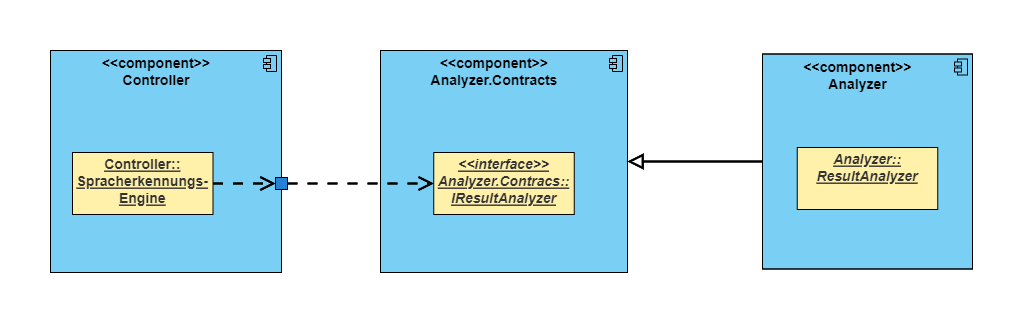
\includegraphics[width=16cm]{compcomp.png}
	\caption{Composite Components}
	\label{fig:compcomp}
\end{figure}
\FloatBarrier

\section{Dependency Injection}
\label{sec:dependencyinjection}
Ein Entwurfsmuster aus der Objektorientierung ist die \gls{di}, also Abhängigkeitsinjektion. Es soll Abhängigkeiten entkoppeln und auf ein Minimum reduzieren. Dabei handelt es sich um eine Weiterentwicklung der \textit{Inversion of Control} aus 2004 durch Martin Fowler \cite{Fowler.2004}. Konkret umgesetzt wird dies durch eine Fabrik oder einen Container, in welchen Objekte zentral erzeugt werden. Dieser injiziert diese dann passend, wenn benötigt. Folgend ein Beispiel:

\begin{figure}[!htb] 
	\centering
	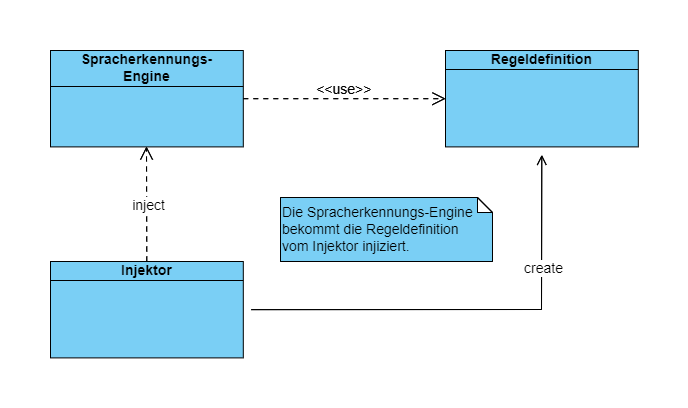
\includegraphics[width=12cm]{dependency_injection.png}
	\caption{Dependency Injection}
	\label{fig:dependency_injection}
\end{figure}
\FloatBarrier

Im Beispiel (siehe \autoref{fig:dependency_injection}) braucht die \textit{Spacherkennungsengine} eine Instanz der \textit{Regeldefinition}. Diese wird zentral im Injektor erzeugt und ihr dann injiziert. Dazu wird zwischen drei Methoden unterschieden \cite{Fowler.2004}, im Unternehmen \gls{arburg} wird folgende genutzt:
\begin{itemize}
	\item Constructor Injection: Die Abhängigkeit wird direkt im Konstruktor als Argument übergeben. 
\end{itemize}

Die Objekte müssen dabei einmalig dem \gls{di}-Container zugewiesen werden. Dies sieht folgendermaßen aus.

\begin{lstlisting}[caption=Dependency Injection, label=lst:depInj]
	this.ExportPart<ISpeechAssist, SpeechAssist>().AsSingleton();
	this.ExportPart<ITextResourcesExtractor, TextResourcesExtractor>();
	this.ExportPart<ITokenHolder, TokenHolder>().AsSingleton();
	this.ExportPart<IResultAnalyzer, ResultAnalyzer>();
\end{lstlisting}

Gemäß dem Dependency Inversion Prinzip (siehe \autoref{sec:compositecomponents}) wird jeder Implementierung eine Abstraktion zugeordnet. Die Instanzen können als einmalig, also als Singleton, definiert werden, um immer das gleiche Objekt zu nutzen. 
	\begin{comment}
	\include{04_Content/theo_grundlagen}
	\include{04_Content/anforderungen}
	\include{04_Content/framework_vergleich}
	\include{04_Content/konzeptionierung}
	\include{04_Content/implementierung}
	\include{04_Content/problemloesung}
	\include{04_Content/performance}
	\include{04_Content/schluss}
	\end{comment}
	
	% Nummerierung wieder auf Römisch und dort weitermachen, wo vorher aufgehört wurde
	\pagenumbering{Roman}
	\setcounter{page}{\theTmpPage}
	\printbibliography
	% Aufzählung Sections ändern
	
	\appendix
	%%%%%%%%%%%%%Anhang%%%%%%%%%%%%%%%%%%
\chapter*{Anhang}
\addcontentsline{toc}{chapter}{Anhang} % Durch das * ohne Nummerierung, muss dafür mit diesem Command extra ins TOC aufgenommen werden
\label{anhang}
\renewcommand{\thesection}{A} % Buchstaben statt Nummern, manuell für jede Section im Anhang

\section{Sprachen der Steuerung}
\label{anh_sec:steuerung_sprachen}
In der Steuerung sind momentan folgende Sprachen verfügbar: 

\begin{longtable}[h]{ | p{5cm} | P{2cm} | }	\hline
	\label{table:sprachen_steuerung}
	\small
	\renewcommand{\arraystretch}{1.5}
	\setlength{\arrayrulewidth}{0.4mm}
	\vspace{.75\baselineskip}
	\cellcolor{Gray0}\textbf{Sprache} & \cellcolor{Gray0}\textbf{Kürzel} \\
	\hline		
	Deutsch						& de-DE \\
	\hline
	Bulgarisch 					& bg-BG \\
	\hline
	Portugiesisch (Brasilien)	& pt-BR \\
	\hline
	Tschechisch 				& cs-CZ \\
	\hline
	Dänisch						& da-DK \\
	\hline
	Griechisch 					& el-GR \\
	\hline
	Englisch (GB)				& en-GB \\
	\hline
	Spanisch					& es-ES \\
	\hline
	Estnisch					& et-EE \\
	\hline
	Finnisch					& fi-FI \\
	\hline
	Französisch					& fr-FR \\
	\hline
	Kroatisch					& hr-HR \\
	\hline
	Ungarisch					& hu-HU \\
	\hline
	Italienisch					& it-IT \\
	\hline
	Japanisch					& ja-JP \\
	\hline
	Koreanisch					& ko-KR \\
	\hline
	Litauisch					& lt-LT \\
	\hline
	Lettisch					& lv-LV \\
	\hline
	Norwegisch 					& no-NO \\
	\hline
	Niederländisch				& nl-NL \\
	\hline
	Polnisch					& pl-PL \\
	\hline
	Rumänisch					& ro-RO \\
	\hline
	Russisch					& ru-RU \\
	\hline
	Slowakisch					& sk-SK \\
	\hline
	Slowenisch					& sl-SL \\ 
	\hline
	Serbisch					& sr-RS \\
	\hline
	Schwedisch					& sv-SE \\
	\hline
	Türkisch					& tr-TR \\
	\hline
	Vietnamesisch				& vi-VN \\
	\hline
	Chinesisch					& zh-CN \\
	\hline
	\caption{In der Steuerung verfügbare Sprachen und ihre Kürzel}
\end{longtable}
\pagebreak % Anhang, kann auch in einzelne Dateien unterteilt werden wenn gewollt
\end{document}
